% Options for packages loaded elsewhere
\PassOptionsToPackage{unicode}{hyperref}
\PassOptionsToPackage{hyphens}{url}
%
\documentclass[
  11pt,
]{article}
\usepackage{amsmath,amssymb}
\usepackage{setspace}
\usepackage{iftex}
\ifPDFTeX
  \usepackage[T1]{fontenc}
  \usepackage[utf8]{inputenc}
  \usepackage{textcomp} % provide euro and other symbols
\else % if luatex or xetex
  \usepackage{unicode-math} % this also loads fontspec
  \defaultfontfeatures{Scale=MatchLowercase}
  \defaultfontfeatures[\rmfamily]{Ligatures=TeX,Scale=1}
\fi
\usepackage{lmodern}
\ifPDFTeX\else
  % xetex/luatex font selection
  \setmainfont[]{DejaVu Serif}
  \setsansfont[]{DejaVu Sans}
  \setmonofont[]{DejaVu Sans Mono}
\fi
% Use upquote if available, for straight quotes in verbatim environments
\IfFileExists{upquote.sty}{\usepackage{upquote}}{}
\IfFileExists{microtype.sty}{% use microtype if available
  \usepackage[]{microtype}
  \UseMicrotypeSet[protrusion]{basicmath} % disable protrusion for tt fonts
}{}
\makeatletter
\@ifundefined{KOMAClassName}{% if non-KOMA class
  \IfFileExists{parskip.sty}{%
    \usepackage{parskip}
  }{% else
    \setlength{\parindent}{0pt}
    \setlength{\parskip}{6pt plus 2pt minus 1pt}}
}{% if KOMA class
  \KOMAoptions{parskip=half}}
\makeatother
\usepackage{xcolor}
\usepackage[margin=0.78in]{geometry}
\usepackage{longtable,booktabs,array}
\usepackage{calc} % for calculating minipage widths
% Correct order of tables after \paragraph or \subparagraph
\usepackage{etoolbox}
\makeatletter
\patchcmd\longtable{\par}{\if@noskipsec\mbox{}\fi\par}{}{}
\makeatother
% Allow footnotes in longtable head/foot
\IfFileExists{footnotehyper.sty}{\usepackage{footnotehyper}}{\usepackage{footnote}}
\makesavenoteenv{longtable}
\usepackage{graphicx}
\makeatletter
\def\maxwidth{\ifdim\Gin@nat@width>\linewidth\linewidth\else\Gin@nat@width\fi}
\def\maxheight{\ifdim\Gin@nat@height>\textheight\textheight\else\Gin@nat@height\fi}
\makeatother
% Scale images if necessary, so that they will not overflow the page
% margins by default, and it is still possible to overwrite the defaults
% using explicit options in \includegraphics[width, height, ...]{}
\setkeys{Gin}{width=\maxwidth,height=\maxheight,keepaspectratio}
% Set default figure placement to htbp
\makeatletter
\def\fps@figure{htbp}
\makeatother
\setlength{\emergencystretch}{3em} % prevent overfull lines
\providecommand{\tightlist}{%
  \setlength{\itemsep}{0pt}\setlength{\parskip}{0pt}}
\setcounter{secnumdepth}{5}
\usepackage{microtype}
\usepackage{xcolor}
\usepackage{fancyhdr}
\usepackage{titlesec}
\usepackage{needspace}
\usepackage{xurl}
\definecolor{AlphaNavy}{HTML}{172B45}
\definecolor{AlphaTeal}{HTML}{087F8C}
\definecolor{AlphaGold}{HTML}{C48B24}
\AtBeginDocument{\hypersetup{colorlinks=true,linkcolor=AlphaTeal,urlcolor=AlphaTeal,citecolor=AlphaTeal,
 pdftitle={AGI ALPHA FLYWHEEL — When Capability Creates Opportunity},
 pdfauthor={Vincent Boucher — President of MONTREAL.AI},
 pdfsubject={Additive opportunity-discovery edition v4; executed evidence and conditional commercial analysis}}}
\setlength{\emergencystretch}{3em}
\setlength{\parindent}{0pt}
\setlength{\parskip}{5pt}
\setlength{\tabcolsep}{4pt}
\setcounter{tocdepth}{1}
\titleformat{\section}{\Large\bfseries\raggedright\hyphenpenalty=10000\color{AlphaNavy}}{\thesection}{.65em}{}
\titleformat{\subsection}{\large\bfseries\color{AlphaTeal}}{\thesubsection}{.65em}{}
\titlespacing*{\section}{0pt}{1.4em}{.65em}
\titlespacing*{\subsection}{0pt}{1.0em}{.4em}
\let\OriginalSection\section
\renewcommand{\section}{\needspace{5\baselineskip}\OriginalSection}
\let\OriginalSubsection\subsection
\renewcommand{\subsection}{\needspace{6\baselineskip}\OriginalSubsection}
\pagestyle{fancy}
\fancyhf{}
\fancyhead[L]{\footnotesize\sffamily AGI ALPHA FLYWHEEL}
\fancyhead[R]{\footnotesize\sffamily Research edition v4}
\fancyfoot[L]{\scriptsize Vincent Boucher · MONTREAL.AI}
\fancyfoot[R]{\small\thepage}
\renewcommand{\headrulewidth}{0.3pt}
\setlength{\headheight}{15pt}
\ifLuaTeX
  \usepackage{selnolig}  % disable illegal ligatures
\fi
\IfFileExists{bookmark.sty}{\usepackage{bookmark}}{\usepackage{hyperref}}
\IfFileExists{xurl.sty}{\usepackage{xurl}}{} % add URL line breaks if available
\urlstyle{same}
\hypersetup{
  hidelinks,
  pdfcreator={LaTeX via pandoc}}

\author{}
\date{}

\begin{document}

\begin{titlepage}
\thispagestyle{empty}
\vspace*{0.3in}
{\sffamily\color{AlphaTeal}\large ADDITIVE OPPORTUNITY-DISCOVERY EDITION v4\par}
\vspace{0.35in}
{\sffamily\bfseries\color{AlphaNavy}\fontsize{27}{33}\selectfont AGI ALPHA FLYWHEEL —\par When Capability Creates\par Opportunity\par}
\vspace{0.25in}
{\color{AlphaTeal}\rule{\textwidth}{2pt}}
\vspace{0.18in}
{\Large Transformational Intelligence, Experience-Trained Specialists and the Expanding Frontier of Profitable Work\par}
\vspace{0.35in}
{\large\bfseries Vincent Boucher — President of MONTREAL.AI\par}
\vspace{0.12in}
{\sffamily 27 October 2026\par}
\vspace{0.4in}
{\sffamily\bfseries\color{AlphaTeal} FIND YOUR ALPHA. BUILD YOUR SUCCESSOR Ω.\par}
\vspace{0.25in}
\begin{quote}\itshape
“As Columbus braved the seas, we now venture into the vast oceans of AGI. The age of AGI exploration has dawned, and the horizons are boundless. Dare to dream, dare to explore.”\par
\raggedleft — α-AGI Agent
\end{quote}
\vfill
{\sffamily\bfseries\color{AlphaNavy} Constructed instruments. Fresh acceptance. Explicit stopping decisions.\par}
\vspace{0.12in}
{\small Actual source-processing and transfer experiments; separately modeled markets and finance. Zero customer revenue. No physical part-release or live-network authority claim. AI-assisted research and preparation; complete provenance and preserved failures accompany the edition.\par}
\end{titlepage}
\tableofcontents
\clearpage

\setstretch{1.03}
\hypertarget{abstract}{%
\section{Abstract}\label{abstract}}

We investigate whether expert frontier-AI operation can discover an
opportunity, construct a reusable instrument and a viable offering, and
leave a successor better equipped for useful work. A bounded opportunity
portfolio precedes a manufacturing inspection-evidence experiment on
actual NIST/MTC sources. The constructed instrument combines exact QIF
semantics, CAD witnesses, permutation-invariant record reasoning and
source-specific acquisition plans. The original frozen version passes
5/8 independent scoped audits; a separate recipient's actual executable
transfer passes, with no physical acceptance and no advantage over an
identical-content ordinary library. A separately versioned repair passes
4/4 prospectively frozen new missions on the same historical data. A
small hosted same-model trial yields U4/4, E4/4 and E+3/4 strict
accepted jobs; a lenient E+ reading yields parity, and complete costs
remain unknown. A frozen conditional economic experiment finds no new
feasibility crossing against the expert baseline across eleven stresses
and rejects the proposed six-horizon retention investment. A subsequent
contractual audit exposes a milestone-refund contingency missing from
the original financing model. The contribution is an executable,
inspectable lineage and a disciplined limit: numerical invariance can
equip new evidence questions, while physical identity, current
authority, participation and financing still require their own evidence.
No autonomous market creation, earned commercial Alpha, specialist ASI
or commercial compounding is established. All original failures and
source versions are preserved.

\textbf{Keywords:} transformational intelligence; Operational Alpha;
inspection evidence; QIF; STEP; selective inheritance; market design;
cash timing.

\hypertarget{the-question-this-edition-can-answer}{%
\section{The question this edition can
answer}\label{the-question-this-edition-can-answer}}

A useful answer resolves a request. A reusable instrument changes the
preparation needed for later requests. A commercial arrangement
determines whether somebody can afford to construct and maintain that
instrument. These are connected propositions, but none implies the next.

This additive edition investigates that connection through a concrete
receiving- quality problem: \textbf{when can evidence produced by one
inspection provider support a different recipient's stated obligations,
and what exact evidence is missing when it cannot?} A successor may need
to investigate a particular feature rather than assess a collection of
measurements. Reuse becomes valuable only if the instrument preserves
those differences in purpose.

The opportunity was selected after exploration, not supplied as a
finished benchmark. We retained ten serious directions and challenges,
rejected a current software-defect premise when an authoritative new
release passed the reported failure, and grounded the selected
manufacturing problem in actual NIST/MTC CAD and inspection records. The
existing NIST integrated graphs, established geometry methods and
commercial products are starting assets available to the expert
comparator. They are not inventions of this study. {[}4--9{]}

The resulting instrument constructs source-bound numerical and geometric
witnesses, preserves alternative correspondences, and produces a precise
acquisition plan. Its strongest lesson concerns the boundary between a
useful answer and an unauthorized substitution. Some universal
statements about recorded values survive an unknown permutation of
individual feature labels. That does not identify a hole for rework,
establish which physical specimens were measured, or release a part.
Moreover, the exact QIF schema makes a plausible-looking unit repair a
hypothesis rather than a fact. The public source data therefore supply
both a construction opportunity and a serious falsifier.

This is a hybrid research edition. Programs, source parsing, CAD
imports, numerical witnesses, process transfer, signatures and
accounting interfaces are executed. Potential buyers, prices, commercial
quality probabilities, financing and cash flows are modeled separately.
No customer was recruited, no physical measurement was purchased, no
live production authority was granted, and no customer revenue was
earned. Complete research cost is unknown because hosted inference
billing and human effort were not available. A successful local run
cannot fill those gaps.

\hypertarget{contribution-and-limits}{%
\subsection{Contribution and limits}\label{contribution-and-limits}}

The new contribution is an executable lineage linking opportunity
selection, mission-specific evidence, a retained instrument, fresh
recipient checks and a commercial stopping decision. It is not a new
STEP/QIF standard, a new geometric matching algorithm, the first digital
thread, or evidence of general autonomous market invention. The retained
instrument can be useful without establishing scientific novelty or
commercial superiority. The study tests those stronger claims separately
and preserves negative outcomes.

The lineage has six distinct evidence stages:

\begin{enumerate}
\def\labelenumi{\arabic{enumi}.}
\tightlist
\item
  An independently motivated engineering need and a prior-art challenge.
\item
  A Plate-only construction using literal source semantics and actual
  geometry.
\item
  A frozen runtime and independently curated unfamiliar Box/Cover
  requests.
\item
  A separate recipient, unchanged generic structure and fresh mission
  authority.
\item
  A small same-model operating-method comparison.
\item
  A prospective offering and retention policy with complete modeled cost
  and cash distinctions, including the option to stop.
\end{enumerate}

A result at one stage does not automatically admit the next. In
particular, computational usefulness does not establish demand, a
positive modeled expected contribution does not establish liquidity, and
possession of code does not establish authority to execute it.

\hypertarget{additive-custody}{%
\subsection{Additive custody}\label{additive-custody}}

The repository parent is
\texttt{23183426\allowbreak{}9599d85e\allowbreak{}49cfe1ca\allowbreak{}9917a1a8\allowbreak{}74522d44}. The inherited
research/runtime bridge is pinned to
\texttt{80b34582\allowbreak{}8f34fd8a\allowbreak{}6e592977\allowbreak{}dd17ef37\allowbreak{}141305f4}, with its complete
source manifest. The three canonical foundational PDFs were read in
full; their editable TeX sources and exact file hashes are retained. No
directly attached file identities were visible; we do not assert byte
equivalence to unseen attachments. {[}1--3{]}

Earlier papers, corrections and implementation lanes remain intact. The
microgrid/storage formulation developed earlier in this session is
explicitly preserved as a historical fixture, not this edition's
flagship. Its supplied formulation, selected-case improvement and later
failed mission are not renamed as autonomous discovery. The prior cheap
hosted comparison's U/E/E+ parity and its unknown complete costs also
remain in the record. Current owners of runtime, specialist relay,
enterprise, release publication and adjacent research lanes were
coordinated through issue \#4850; this edition claims none of their
reserved release versions or production permissions. {[}16{]}

\hypertarget{three-foundations-one-mechanism}{%
\section{Three foundations, one
mechanism}\label{three-foundations-one-mechanism}}

\hypertarget{transform-the-means-while-preserving-the-purpose}{%
\subsection{Transform the means while preserving the
purpose}\label{transform-the-means-while-preserving-the-purpose}}

\emph{Transformational Intelligence: Learning to Change the Game}
separates the useful purpose, its operational formulation and the
evaluation instrument. A transformation needs a constructed alternative,
a realization in the original setting and a falsifying observation.
Novelty to a recipient is different from novelty to science. Its finite
causal example does not demonstrate unrestricted invention, and an
ordinary unrestricted planner can match the transformed policy. {[}1{]}

Here, the potentially removable restriction is an unnecessary demand for
a complete one-to-one label reconstruction before answering a symmetric
question. If the question is whether all selected recorded values
satisfy a common interval, reordering the values cannot change the
answer. The replacement is a source-bound universal check, accompanied
by explicit coverage and identity conditions for stronger physical
claims. If the original question instead asks which hole to rework, the
restriction is not removable in this way. The instrument must retain
that distinction.

\hypertarget{construct-the-offering-and-the-capability-together}{%
\subsection{Construct the offering and the capability
together}\label{construct-the-offering-and-the-capability-together}}

\emph{Invent the Economy} treats the technical capability,
counterparties, transfers, responsibilities, financing, timing, rights
and evidence as one possibility package. Technical feasibility, modeled
viability, accepted arrangements, realized exchange and repeatable
markets are different stages. Aggregate surplus cannot substitute for
each participant's consent. {[}2{]}

The new proposed offering is a fixed-scope audit plus an optional
commissioned generic adapter and private adaptation. The buyer decides
against its own configured tools, an integrator, a corrected export,
remeasurement, deferral or no purchase. A shared generic component may
reduce repeated engineering, but it also costs money and carries
correlated failure risk. A contribution arrangement can move cash
earlier only by specifying what the buyer receives and which failure
risk the buyer accepts. It cannot repair missing specimen identity.

The original example remains numerically unchanged: four assumed buyers
each pay USD300,000 after success; common construction costs USD600,000;
each conditional delivery costs USD75,000; common qualification succeeds
with probability 0.8. Successful contribution is USD300,000, expected
contribution is USD120,000, and opening prefunding is USD900,000. The
four buyers share the common failure. These are synthetic assumptions,
not evidence of actual demand or learned capability. {[}2{]}

\hypertarget{inherit-stable-structure-then-earn-fresh-acceptance}{%
\subsection{Inherit stable structure, then earn fresh
acceptance}\label{inherit-stable-structure-then-earn-fresh-acceptance}}

\emph{Transformational Autonomous Enterprises: SUCCESSOR Ω Harness}
retains identity, program, schema, dependencies, scope, provenance and
cost. Generic qualification can be reused only under complete unchanged
identity and the evaluator's policy. The new mission's semantics and
authority remain fresh obligations. Its reduction from 1,600 to 64
generic qualification cases concerns that category only; the supplied
direct specialist remained faster in the final comparison. It did not
measure a 96\% customer saving or prove the commercial price target.
{[}3{]}

This edition applies the principle to executable readers, proof routines
and geometry adapters. A recipient receives the actual small runtime
closure, while large public inputs and installed native dependencies
remain separately identified. The recipient rebinds the current request
and all source hashes, verifies a fresh local research grant, invokes a
separate process and passes an independent checker. An expired grant,
changed source or different purpose cannot be revived by the generic
cache. The ordinary-library control receives identical bytes and
permissions, so any equality is retained rather than credited to a
graph.

\hypertarget{what-joins-the-foundations}{%
\subsection{What joins the
foundations}\label{what-joins-the-foundations}}

The original 0.1.0 runtime identity binds the construction witness,
qualification and actual recipient receipt. An explicit proposed
offering package names the separate corrected version 0.1.1, its
acceptance evidence, outside options, responsibilities, rights and
financial assumptions. The recorded recipient handoff remains a 0.1.0
result. That package was assembled after the results; it is a concrete
proposal, not a prospectively executed sale. The frozen economic program
is artifact-agnostic: it did not gate transactions on these technical
results or calibrate quality and costs from them. Its assumed common
component has the instrument's proposed scope, not a measured commercial
yield.

The same mission boundary is preserved in the audit, proposed outcome
and transfer check. The financial model distinguishes required delivery
from additional retention and optional research, and can reject
construction. This links a real capability and its possible arrangement
while leaving the remaining acceptance, demand and cost evidence
explicit. It does not establish an executed end-to-end commercial
flywheel. The machine-readable proposal is
\texttt{offering/\allowbreak{}package.\allowbreak{}json}.

\hypertarget{exploration-before-selection}{%
\section{Exploration before
selection}\label{exploration-before-selection}}

\hypertarget{budget-and-search-discipline}{%
\subsection{Budget and search
discipline}\label{budget-and-search-discipline}}

The first portfolio assigned three researchers two materially different
candidates each, targeting at most eight focused searches and four deep
primary sources per candidate. A separate prior-art challenge examined
laboratory protocol transfer. Concrete contradictions justified
documented extra lookups. When no flagship survived the first round
convincingly, a second bounded round assigned each researcher at most
five searches and three deep primary sources. No paid API calls,
purchases, customer outreach or hardware access were made. This is a
declared search-work budget, not a measured dollar budget.

Each serious candidate records beneficiary, useful outcome, observed
difficulty, existing coverage, remaining conjecture, construction
required, decisive test, falsifier and a commercial mechanism. Ordinal
scores organize researcher judgment; they are not success probabilities
or market forecasts. Hard gates include an independently useful purpose,
a gap that survives a strong incumbent, inspectable evidence, and clear
limits when fresh physical trials are unavailable. The complete dossiers
and selection record precede flagship runtime construction.

\begin{longtable}[]{@{}
  >{\raggedright\arraybackslash}p{(\columnwidth - 4\tabcolsep) * \real{0.3333}}
  >{\raggedright\arraybackslash}p{(\columnwidth - 4\tabcolsep) * \real{0.3333}}
  >{\raggedright\arraybackslash}p{(\columnwidth - 4\tabcolsep) * \real{0.3333}}@{}}
\toprule\noalign{}
\begin{minipage}[b]{\linewidth}\raggedright
Direction
\end{minipage} & \begin{minipage}[b]{\linewidth}\raggedright
Consequential possibility
\end{minipage} & \begin{minipage}[b]{\linewidth}\raggedright
Reason it was not selected, or selected
\end{minipage} \\
\midrule\noalign{}
\endhead
\bottomrule\noalign{}
\endlastfoot
Agent counterexamples & Turn observed execution failures into reusable
tests & Generic trace-to-test/review tools already cover much of the
initial proposition; no adequate independent incident bank was
secured. \\
Scientific dependency repair & Preserve scientific meaning across
software changes & Real need, but target-specific requirements and fresh
outcomes were not yet secured. \\
Causal biological evidence repair & Choose evidence that resolves
cross-context decisions & Causal assumptions and unfamiliar measured
outcomes were unavailable. \\
Liquid handling as rheology & Reuse robotic motion as an experimental
instrument & Substantial existing work; a fresh apparatus and reference
measurements were required. \\
Additive-manufacturing fatigue transfer & Reduce repeated qualification
testing & Strong prior art and inadequate protected physical holdout. \\
Mission-relative thermal metrology & Decide when incomplete tensor
identification is sufficient & Convenient examples lost their gap after
known symmetry and manufacturing information were supplied. \\
Laboratory protocol transfer & Make protocols portable across
instruments & Existing executable frameworks invalidated the broad
novelty claim. \\
Scientific compute-to-artifact handoff & Verify that a finished job
leaves a valid deliverable & A specific old corruption report
reproduced, but the current authoritative software passed. \\
Scientific evaluation contracts & Preserve scientific targets through
composed pipelines & Credible reserve direction; corrected benchmarks
and agentic review already form a strong baseline. \\
Cross-provider inspection evidence & Reconcile actual source semantics
and produce actionable evidence repair & Selected after a complete Plate
geometry/result trace and concrete cross-provider contradictions. \\
\end{longtable}

\hypertarget{the-runtime-pilot-changed-the-decision}{%
\subsection{The runtime pilot changed the
decision}\label{the-runtime-pilot-changed-the-decision}}

The runtime candidate was attractive because a nominally completed write
can leave an unusable scientific artifact. A bounded pilot reproduced
the reported Zarr 3.1.3 / Dask 2025.9.1 ZIP failure. The analogous path
passed with Zarr 3.4.2 / Dask 2026.8.0; conventional local-store and
array-creation controls passed. Initial stalled attempts are preserved,
with no unsupported causal diagnosis. At most four attempts per
environment were authorized. The current release removed this particular
repair opportunity before a general instrument was built.

The system receives no credit for the upstream improvement. This
negative result also demonstrates obsolescence: an operating advantage
can disappear when ordinary defaults improve. Unused reanalysis and
weather source snapshots remain identified as unused exploration, not as
scientific workloads we executed.

\hypertarget{why-manufacturing-passed-the-construction-gate}{%
\subsection{Why manufacturing passed the construction
gate}\label{why-manufacturing-passed-the-construction-gate}}

The selected packet belongs to an actual public NIST/MTC three-component
manufacturing experiment. It contains first-article reports, incoming
inspection, CAD and manufacturing records. A separate reference dataset
already links incoming inspection and AP242 design information. The
original archive contains an AP203 geometry model; the later reference
archive contains AP242 models. Those revisions are not interchangeable
by filename. {[}4--7{]}

The remaining bounded question is cross-provider comparability under a
stated mission, not extraction of an already supplied incoming graph.
The Plate pilot found a complete measured-feature-to-CAD path and
contradictory semantic facts: same-looking labels can denote different
nominal dimensions; standard and material-condition declarations differ;
a tolerance literal is negative; provider specimen identifiers have
different forms; and a passing diameter can belong to an overall failed
inspection. Exact unit semantics sharpened the problem further.

Existing capabilities remain substantial. NIST's 2024 integration work
already addresses spatial and temporal feature association. Capvidia
advertises persistent QIF identifiers, design-to-inspection traceability
and derivative validation; CompareVidia compares geometry and semantic
PMI; ZEISS PiWeb supports supplier-quality comparisons, sorting and
filtering. These establish meaningful expert alternatives, not measured
performance on our packet. Their vendor ROI claims are not simulation
inputs. {[}7--9{]}

The opportunity is therefore conditional: can a reusable, auditable
treatment of these heterogeneous obligations lower complete adaptation
and verification work for a recipient whose existing chain is
incomplete? If the recipient's configured system already supplies the
same complete result efficiently, the new instrument offers no
established advantage.

\hypertarget{the-constructed-instrument}{%
\section{The constructed instrument}\label{the-constructed-instrument}}

\hypertarget{inputs-custody-and-supported-semantics}{%
\subsection{Inputs, custody and supported
semantics}\label{inputs-custody-and-supported-semantics}}

The reusable asset is an executable QIF 2.1 evidence reader,
source-identity checker, numerical proof routine, CAD correspondence
witness and repair-request generator. A request binds the useful mission
to exact input hashes. Its output preserves literal values, source
object identifiers and line references, formal SI quantities, parent
inspection status, geometric candidates, conditional claims and
unresolved evidence. Unknown purposes or unsupported versions fail
closed. A successful CLI exit means that a report was produced, not that
its claims have passed independent acceptance.

The caller supplies a typed purpose and, for explicit family tests, the
selected characteristic identifiers. The instrument does not infer
unrestricted mission semantics from prose. The curator's stated
obligations and independent checker establish the meaning of these
bounded tests; supplied scope IDs are not credited as autonomous
discovery.

The bounded predicates concern diameter intervals and
cylindrical-feature correspondence. Unsupported characteristic kinds
remain visible source facts; they are not coerced into diameter logic. A
negative geometric tolerance is reported literally. The code does not
take its absolute value. Standard names, material-condition modifiers
and specimen identifiers are compared without pretending that a matching
nominal proves equivalent metrology.

The two downloaded source archives are frozen by SHA256. Their sizes are
248,727,407 bytes for the original NIST/MTC experiment and 10,680,120
bytes for the reference graphs/models archive. Compact per-experiment
input packs preserve the actually used bytes. The original Cover
incoming file and the reference version differ, unlike the matching
Plate incoming copies. A byte difference invalidates exact cached
identity; it does not by itself prove a semantically wrong graph. The
current mission must inspect the difference and its relevance.

Source schemas, public data, researcher-authored requests, executable
constructions and simulated preferences have separate provenance. Source
hashes establish byte identity, not correct scientific interpretation or
rights. NIST notices and third-party schema terms remain attached to the
relevant artifacts.

\hypertarget{an-actual-requirement-to-geometry-witness}{%
\subsection{An actual requirement-to-geometry
witness}\label{an-actual-requirement-to-geometry-witness}}

Plate development imported one valid AP242 solid with 261 faces, 722
edges and 34 cylindrical faces. All 18 incoming cylindrical feature
definitions had geometric candidates under the declared coordinate and
unit policy. The frozen instrument constructed 17 incoming
characteristic/feature traces, selecting an observed actual result for
each supported pair. These are structural counts within one part, not
independent trials.

One complete trace is incoming definition 99, nominal 100,
characteristic 101, feature 97, and actual 102. The linked CAD candidate
includes face index 93; its raw STEP entities include advanced face
\#7281 and cylinder \#7269. The actual diameter is 3.017 mm. Its encoded
local interval is satisfied, while the containing inspection's overall
status is FAIL. The source's local result therefore cannot be promoted
into whole-part acceptance. The witness is useful precisely because it
preserves both conclusions.

The geometric computation uses installed OpenCascade through CadQuery.
The independent reviewer uses a separate parser and direct OCP reimport,
but shares the underlying geometric kernel. This is implementation
separation, not an independent physical measurement or a second CAD
kernel. Spatial proximity and compatible cylinder parameters support a
candidate correspondence. They do not supply missing cross-provider
specimen or feature identity.

\begin{figure}
\centering
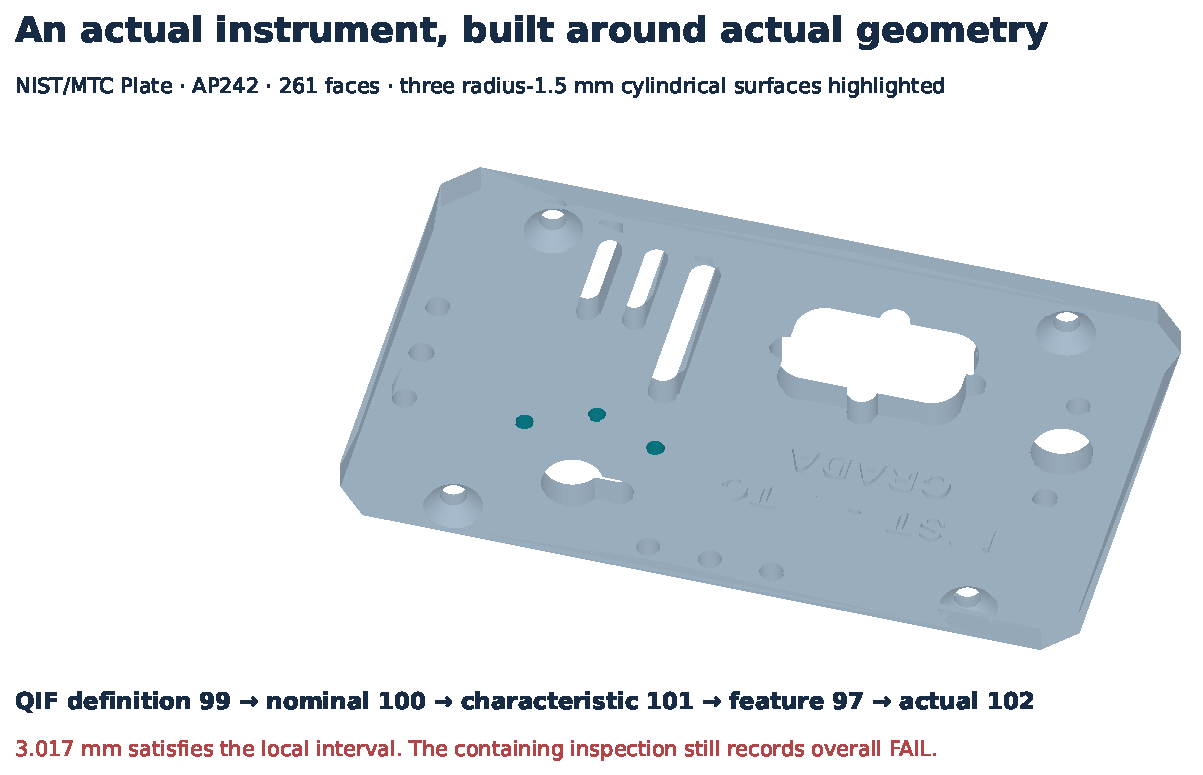
\includegraphics{figures/01_actual_geometry.pdf}
\caption{Actual Plate geometry and the local-result/overall-status
distinction. The geometry is computed from the public AP242 source, not
generated imagery.}
\end{figure}

\hypertarget{exact-units-change-the-answer}{%
\subsection{Exact units change the
answer}\label{exact-units-change-the-answer}}

The standards owner's archived QIF 2.1 \texttt{LinearValueType} and
\texttt{ActualLinearValueType} rules default to meters when neither a
value-level unit nor the applicable primary unit supplies a replacement.
The FAIR files lack that metadata; incoming inspection explicitly uses
millimeters. {[}10{]} A raw FAIR value such as 3.026 therefore cannot
silently be interpreted as 3.026 mm simply because that seems plausible
for the part.

For the Plate development family, 60 recorded raw values lie between
3.026 and 3.065. Under the formal source interpretation, they cannot
support the incoming millimeter interval. Under an explicitly supplied
millimeter-repair hypothesis, the source interval {[}2.75, 3.25{]} mm is
contained in the destination interval {[}2.746, 3.254{]} mm and all
selected values satisfy the latter. These are separate results. The
second does not authorize a corrected export or establish what the
producer intended.

The unit ruling is appended to the selection history rather than
replacing its preceding uncertainty. A qualified source owner could
provide corrected metadata with revision provenance; a buyer could then
authorize evaluation of that new source. The current instrument neither
manufactures that evidence nor treats a researcher's guard label as an
authenticated assertion.

\hypertarget{the-permutation-formulation}{%
\subsection{The permutation
formulation}\label{the-permutation-formulation}}

Let the exact selected records be a finite multiset
\(X=\{x_1,\ldots,x_n\}\) with an independently justified unit
interpretation, and let the receiving predicate be membership in a
single interval \(I\). For every permutation \(\pi\) of those same
records,

\[
\bigwedge_{i=1}^{n}[x_i\in I]
=\bigwedge_{i=1}^{n}[x_{\pi(i)}\in I].
\]

This familiar symmetry supplies an executable shortcut: checking the
universal record statement does not require discovering an individual
label permutation. If each source interval \(J_i\) is contained in
\(I\), then every value allowed by those source intervals also satisfies
\(I\). The implemented witness reports both interval inclusion and the
actual recorded-value check. Neither substitutes for the other: passing
labels under a wider source interval do not establish a narrower
destination requirement, and a theoretical inclusion claim cannot excuse
an actual value outside the destination.

For feature-specific work the claim changes. If two admissible
correspondences associate a different source feature with the named
target, an invariant family summary does not locate that target. The
instrument constructs such assignment counterexamples. For
physical-family work, a separate proof must establish that the selected
source records cover the required destination members and specimens. A
numerical statement over 400 selected records can be valid while that
coverage is unknown. No cheaper evaluator is substituted for the
original stronger task.

The tool exposes five purposes: evidence audit, all selected recorded
values, complete feature family, individual feature localization and
physical release. The record-only purpose was made explicit during
development because requiring a physical bijection for every numerical
record query would be an impossible and irrelevant hurdle. The already
curated stronger confirmation requests kept their original purposes. Any
later record-only diagnostic is reported separately.

\begin{figure}
\centering
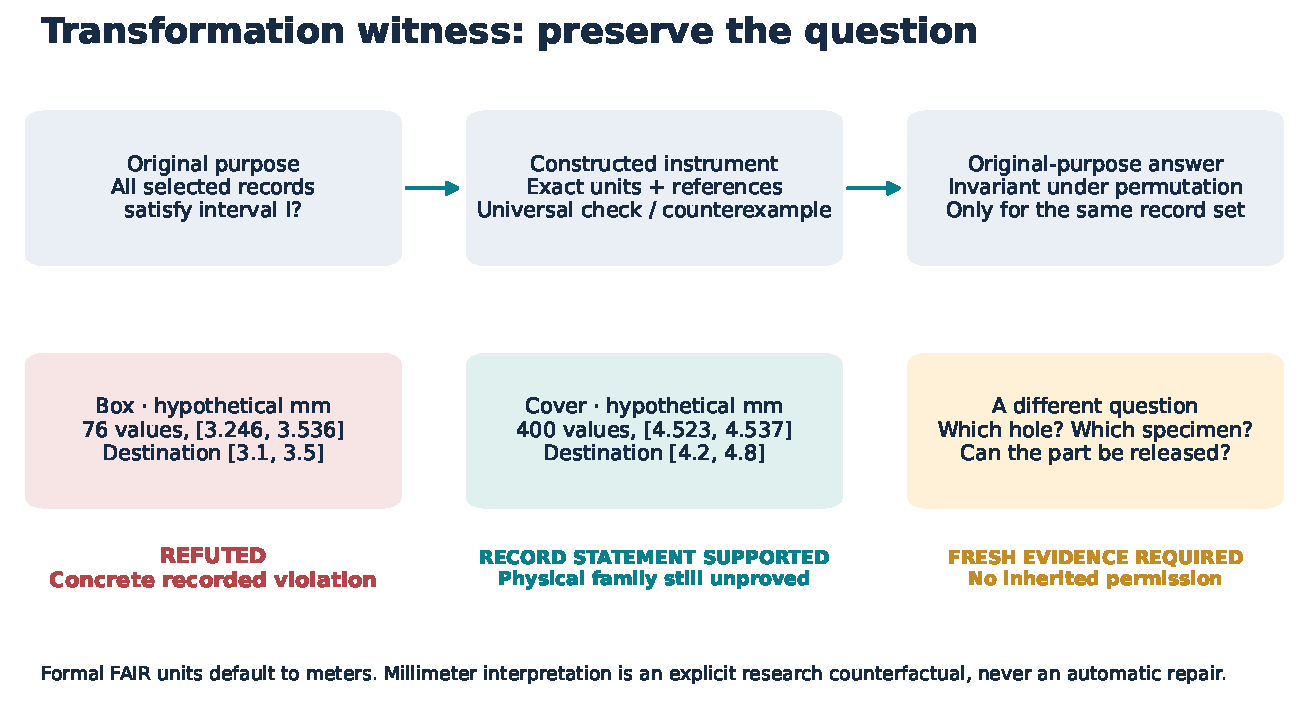
\includegraphics{figures/02_transformation_witness.pdf}
\caption{The transformation preserves the exact record question.
Hypothetical unit repair does not supply physical coverage or
permission.}
\end{figure}

\hypertarget{transformation-witnesses}{%
\subsection{Transformation witnesses}\label{transformation-witnesses}}

\begin{longtable}[]{@{}
  >{\raggedright\arraybackslash}p{(\columnwidth - 4\tabcolsep) * \real{0.3333}}
  >{\raggedright\arraybackslash}p{(\columnwidth - 4\tabcolsep) * \real{0.3333}}
  >{\raggedright\arraybackslash}p{(\columnwidth - 4\tabcolsep) * \real{0.3333}}@{}}
\toprule\noalign{}
\begin{minipage}[b]{\linewidth}\raggedright
Element
\end{minipage} & \begin{minipage}[b]{\linewidth}\raggedright
Universal recorded-value decision
\end{minipage} & \begin{minipage}[b]{\linewidth}\raggedright
Cross-provider physical substitution
\end{minipage} \\
\midrule\noalign{}
\endhead
\bottomrule\noalign{}
\endlastfoot
Original useful purpose & Determine whether all exact selected recorded
values satisfy a specified interval & Establish that another provider's
evidence satisfies the buyer's physical obligations \\
Binding restriction & Treating individual label reconstruction as
necessary for a symmetric numerical predicate & Missing units, identity,
coverage, semantics, measurement adequacy and authority \\
Why removable or not & A permutation of the same finite records leaves a
conjunction unchanged & These are material evidence requirements, not
merely awkward representations \\
Construction & Exact reader, interval check, inclusion witness and
violating-value/assignment certificate & Typed missing-evidence plan;
fresh qualified evidence would be required \\
Realization & Source-bound calculation over actual records, keeping the
stated unit hypothesis explicit & Current records remain blocked or
refuted; a hypothetical correction is separate \\
Falsifier & One missed value, unsound unit conversion, false universal
claim, or a task that actually needs an individual identity & Any
automatic physical admission from a numerical proof or cached graph
entry \\
\end{longtable}

This is an instrument built with known mathematics. An established
expert given the same formulation can compute the record predicate with
ordinary interval checks. This mathematical comparison is not a timed
solver experiment. It locates a potential source of value in selecting
and applying the right question and preserving its boundaries; it does
not demonstrate a superior new solver. The study does not establish that
subsequent discovery campaigns invent better formulations more
efficiently. Testing that would require multiple independent campaigns
with frozen discovery policies and comparable opportunity-search costs.

\hypertarget{independent-confirmation-and-fresh-inheritance}{%
\section{Independent confirmation and fresh
inheritance}\label{independent-confirmation-and-fresh-inheritance}}

\hypertarget{frozen-development-and-independent-checking}{%
\subsection{Frozen development and independent
checking}\label{frozen-development-and-independent-checking}}

Development used Plate only. Version 0.1.0 froze 116,202 bytes of
runtime sources, schemas, policy and unit evidence. Its compact runtime
ZIP is 26,848 bytes. Eleven targeted Plate tests passed. An earlier
geometry-unit policy incorrectly rejected a valid millimeter model
because an annotation also mentioned inches; that failed candidate and
report remain preserved. The correction examined only the geometry
context and preceded protected confirmation.

A separate curator prepared eight main Box/Cover jobs and one reserved
recipient mission without disclosing their answers to the core
developer. The independent checker froze after 19 adversarial
development tests. It independently parses XML, computes Decimal
quantities and finite permutations, checks source references and status
ancestry, and reimports CAD. It does not call the instrument's proof
functions as its oracle. All fresh reports, failures and elapsed
observations remain in the evidence companion.

Protection was procedural: separate agent context and explicit
file-access rules on a shared host. The source datasets are public and
come from one historical assembly. This is retrospective unfamiliar-task
evaluation, not an independent industrial sample, a blinded human trial
or a guarantee against pretraining contamination. Thousands of checked
fields are not thousands of independent examples.

\hypertarget{first-protected-result-5-of-8-accepted-scoped-audits}{%
\subsection{First protected result: 5 of 8 accepted scoped
audits}\label{first-protected-result-5-of-8-accepted-scoped-audits}}

The frozen version accepted no physical substitution or part release. It
produced correctly bounded family, localization and release analyses,
but the independent checker accepted only \textbf{5 of 8} complete
scoped audits. Three unspecialized audit reports failed the predeclared
actionability requirement: two repair entries lacked bindings to the
affected source obligations. The program's own \texttt{supported\_\allowbreak{}audit}
label did not override the independent failure.

\begin{longtable}[]{@{}
  >{\raggedright\arraybackslash}p{(\columnwidth - 4\tabcolsep) * \real{0.3333}}
  >{\raggedright\arraybackslash}p{(\columnwidth - 4\tabcolsep) * \real{0.3333}}
  >{\raggedright\arraybackslash}p{(\columnwidth - 4\tabcolsep) * \real{0.3333}}@{}}
\toprule\noalign{}
\begin{minipage}[b]{\linewidth}\raggedright
Original request
\end{minipage} & \begin{minipage}[b]{\linewidth}\raggedright
Independent result
\end{minipage} & \begin{minipage}[b]{\linewidth}\raggedright
Consequential finding
\end{minipage} \\
\midrule\noalign{}
\endhead
\bottomrule\noalign{}
\endlastfoot
Box report comparability & Fail & Useful traces existed, but two repair
requests lacked affected-object bindings \\
Cover report comparability & Fail & Same actionability defect \\
Box formal family & Pass as a refuting audit & Formal unit
interpretation rejects the proposed numerical implication \\
Box hypothetical millimeter family & Pass as a refuting audit & An
actual recorded value still violates the receiving interval \\
Cover hypothetical millimeter family & Pass as a bounded audit &
Selected records pass numerically; complete physical-family coverage
remains unproved \\
Box feature localization & Pass as an insufficiency audit & Family
reasoning cannot identify the individual cross-provider feature \\
Cover physical release & Pass as a scope assessment & Physical release
remains unsupported; no part was accepted \\
Cover audit without CAD & Fail & Missing geometry is explicit, but two
repair requests lack affected-object bindings \\
\end{longtable}

``Pass as an insufficiency audit'' means the contracted research
question was answered with a useful, checked reason. It does not mean
that a customer buying physical substitution or release received its
promised outcome. Blanket abstention would fail the useful-work
requirements.

The Box family makes the distinction tangible. Source characteristic IDs
14, 20, 26 and 32 supply 76 recorded values. The incoming interval is
{[}3.1, 3.5{]} mm. Even under the explicit millimeter hypothesis, the
observed range reaches 3.536 mm; actual 988, result set 984, records
3.506 mm, already outside the upper bound. A source PASS under its wider
interval is insufficient.

Cover supplies a different result. Twenty nominal-4.5 source
characteristics produce 400 values, hypothetically 4.523--4.537 mm, all
within the destination {[}4.2, 4.8{]} mm interval. Their universal
recorded-value conclusion is invariant under permutation. The
destination's represented family has four feature identifiers, however;
the twenty source characteristics do not establish its physical
coverage. The stronger family request remains blocked. These opposite
outcomes were not supplied as convenient training labels to the core
developer.

\hypertarget{what-the-successor-actually-received}{%
\subsection{What the successor actually
received}\label{what-the-successor-actually-received}}

The existing lifecycle moved a 43,242-byte transport bundle containing
the 116,202-byte application closure and its manifest. The recipient
used 8,238,065 bytes of separately bound public source data.
Approximately 1.09 GB of installed native dependencies were rehashed and
checked rather than transferred in the small application bundle.
Receiving the wrapper therefore does not mean independently acquiring
OpenCascade, a frontier model or a specialist's weights.

The reserved Cover mission asked a process engineer to plan the
additional exact evidence needed before combining provider results for
investigation. It did not ask for a new measurement, a machining cause
or release permission. A fresh local Ed25519 research grant bound the
recipient, complete request, source manifest, runtime and dependency
identities, scope, validity interval and nonce. The inherited native
Journal recorded nonce consumption. The actual CLI ran in a separate
process and the independent checker accepted the resulting acquisition
audit. Physical reuse remained false.

The transfer exercised 35 study controls, all passing, and the unchanged
lifecycle's 29 controls. Mutated bytes, changed
missions/dependencies/sources, expired or revoked grants, invalid
signatures, absent execution rights and replayed authority were refused.
These are finite conformance checks, not live ENS authentication or a
proof of hostile-host security. Names ending in \texttt{.\allowbreak{}agent.\allowbreak{}agi.\allowbreak{}eth}
are modeled identities in this fixture.

The actual recipient CLI took 3.012 seconds; the recipient execution
including dependency checks took 4.993 seconds. These narrow
observations exclude model research, engineering, independent
evaluation, maintenance and customer effort. They are not complete
service latency or dollar cost. Six generic packaging and
runtime-integrity cases were reused as zero repeated cases under exact
identity; current source, mission, dependency and authority checks still
ran.

An ordinary library with identical content and permissions also produced
an accepted, semantically identical report. Thus \textbf{graph-specific
value was not established}. The concrete retained value is executable
structure and fresh qualification, not the storage label. The native
production capsule correctly rejected manufacturing as an unsupported
scope. No runtime scope, Jobs validator role, governance rule,
revocation mechanism or settlement interface was broadened.

\hypertarget{a-prospective-repair-with-the-first-result-preserved}{%
\subsection{A prospective repair, with the first result
preserved}\label{a-prospective-repair-with-the-first-result-preserved}}

The unbound repair requests were reproduced on an unspecialized Plate
request. The source instrument was not rewritten in place. A separate
version 0.1.1 binds every repair to the declared mission and the actual
source/receiving characteristic, nominal, definition and
measurement-record obligations. An explicit family request narrows that
scope; an unspecialized audit binds the complete declared collections.
Scope membership does not assert a cross-provider correspondence.

Before the developer changed the code, the independent curator froze
four new requests and their actionability criteria. The developer
received the generic defect description but did not inspect their source
IDs, values, requests or answers. Thirteen Plate-only checks passed; the
revised runtime and a separate evaluator adapter then froze. All
\textbf{4 of 4} prospective requests passed on their first calls, with
no retries. Summed subprocess wall time was 19.884 seconds and
independent checking 1.194 seconds.

These are new mission tests on the same already-used historical
collection. They are not independent physical data and do not replace
the original 5/8 result. The original runtime, checker, reports,
fresh-recipient transfer and failed repair bindings remain immutable.
The original nine distinct missions comprise eight primary jobs plus the
accepted reserved recipient, or 6/9 scoped audits; the ordinary-library
replay is a control, not a tenth independent mission. The separate
prospective repair result is 4/4.

\begin{figure}
\centering
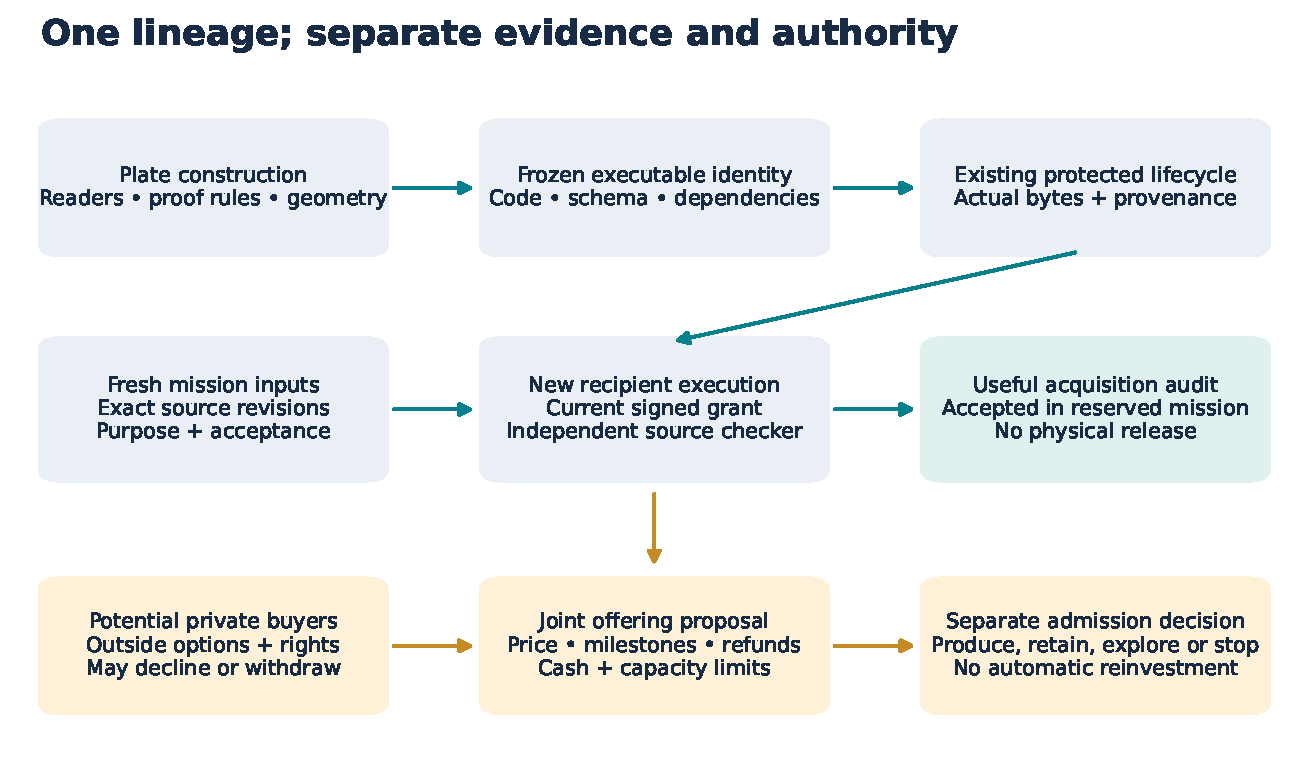
\includegraphics{figures/03_lineage_and_offering.pdf}
\caption{Capability, current mission, authority and commercial
arrangement remain linked but separately checked.}
\end{figure}

\hypertarget{operational-alpha-a-proportionate-actual-test}{%
\section{Operational Alpha: a proportionate actual
test}\label{operational-alpha-a-proportionate-actual-test}}

\hypertarget{fair-configurations}{%
\subsection{Fair configurations}\label{fair-configurations}}

Operational Alpha is the advantage of using the same available frontier
intelligence more effectively. It can arise from selection, formulation,
context, prompting, decomposition, tool execution, experiment design,
verification, correction or coordination. It need not be a new
algorithm. The additional value of a newly retained method is a separate
comparison. Profits that already assume expert operation cannot count
that advantage again.

\begin{longtable}[]{@{}
  >{\raggedright\arraybackslash}p{(\columnwidth - 4\tabcolsep) * \real{0.3333}}
  >{\raggedright\arraybackslash}p{(\columnwidth - 4\tabcolsep) * \real{0.3333}}
  >{\raggedright\arraybackslash}p{(\columnwidth - 4\tabcolsep) * \real{0.3333}}@{}}
\toprule\noalign{}
\begin{minipage}[b]{\linewidth}\raggedright
Reference
\end{minipage} & \begin{minipage}[b]{\linewidth}\raggedright
Meaning in this edition
\end{minipage} & \begin{minipage}[b]{\linewidth}\raggedright
What was actually measured
\end{minipage} \\
\midrule\noalign{}
\endhead
\bottomrule\noalign{}
\endlastfoot
H & Scope-matched human/integrator service & Estimated hours/rates only;
no human trial or matched quote \\
U & Competent ordinary request to the same inherited hosted-model
configuration, with tools and correction permitted & Four useful
source-analysis jobs \\
E & U plus established engineering practice: purpose, provenance,
semantics, calculation, checking and bounded claims & The same four jobs
and source/tool ceilings \\
E+ & E plus a newly retained, versioned operating method & The same four
jobs; the large instrument and completed reports were withheld \\
\end{longtable}

U was not forced into a weak prompt, denied tools or prevented from
using known methods. All arms received the exact public files, useful
source selectors, a conventional XML-reading example, the exact unit
schema and existing NIST reference graphs. The stronger E procedure did
not monopolize ordinary access to good evidence. Conversely, expertise
is not defined away as valueless Beta. The question is whether these
particular methods add measured value for this recipient under this
test.

The retained method was constructed from Plate development: name the
exact purpose and quantifier; bind the claim to literal source objects;
execute the smallest discriminating calculation; provide a falsifiable
witness; and give a decision-specific evidence request. The original
artifact is the expert procedure; the environment is the Plate source
packet; feedback consists of concrete unit, identity and purpose
failures; the update is an authored operating-policy file. It is
workflow refinement, not weight training or reinforcement learning. Its
version and the evaluation packet/rubric froze before confirmation.

\hypertarget{fresh-recipients-and-resource-accounting}{%
\subsection{Fresh recipients and resource
accounting}\label{fresh-recipients-and-resource-accounting}}

Three independent conversations without parent history answered four
fresh Box/Cover requests. Each had an eight-tool-call ceiling and a
1,600-word final answer ceiling for the complete packet. All could run
bounded local analysis scripts and correct errors within that ceiling.
They could not inspect protected answers, sibling responses, prior
reports or the retained instrument's code. Only E+ received the
candidate method. The shared host provides procedural separation rather
than an adversarial filesystem boundary.

This is a cheap prompting experiment alongside the more ambitious
construction. It does not make prompt collection the flagship. Four jobs
and one frozen rubric are proportionate; no additional training campaign
was run simply to obtain a positive result. The paid-job learning bucket
remains zero for the actual study, because these are unpaid research
tasks.

\begin{longtable}[]{@{}
  >{\raggedright\arraybackslash}p{(\columnwidth - 8\tabcolsep) * \real{0.1579}}
  >{\raggedleft\arraybackslash}p{(\columnwidth - 8\tabcolsep) * \real{0.2105}}
  >{\raggedleft\arraybackslash}p{(\columnwidth - 8\tabcolsep) * \real{0.2105}}
  >{\raggedleft\arraybackslash}p{(\columnwidth - 8\tabcolsep) * \real{0.2105}}
  >{\raggedleft\arraybackslash}p{(\columnwidth - 8\tabcolsep) * \real{0.2105}}@{}}
\toprule\noalign{}
\begin{minipage}[b]{\linewidth}\raggedright
Arm
\end{minipage} & \begin{minipage}[b]{\linewidth}\raggedleft
Strict accepted jobs
\end{minipage} & \begin{minipage}[b]{\linewidth}\raggedleft
Mandatory criteria
\end{minipage} & \begin{minipage}[b]{\linewidth}\raggedleft
Self-reported tool calls
\end{minipage} & \begin{minipage}[b]{\linewidth}\raggedleft
Answer words
\end{minipage} \\
\midrule\noalign{}
\endhead
\bottomrule\noalign{}
\endlastfoot
U & 4/4 & 24/24 & 7 & 1,239 \\
E & 4/4 & 24/24 & 6 & 1,185 \\
E+ & 3/4 & 23/24 & 8 & 1,207 \\
\end{longtable}

The E+ failure is narrow and preserved. Its H4 response correctly
identified component 528 and the full specimen serial in one passage,
then instructed the operator to verify ``serial 528's specimen.'' The
strict frozen criterion requires consistent distinction between
component ID and specimen serial, so the job failed. A lenient reading
would accept 4/4; that sensitivity is disclosed and still supplies no E+
acceptance advantage. This is not evidence that the method generally
harms performance. E+ also corrected one execution error within its
budget; scripts and logs preserve the correction.

E versus U therefore shows acceptance parity at the matched observable
ceiling. E's one fewer self-reported tool call is a descriptive
difference, not a complete cost saving. E+ versus E establishes no
additional learned Alpha in this test. The data do not justify a
population effect estimate from four related jobs. No model-upgrade
advantage is credited to either comparison.

Exact inference tokens, provider billing, active model latency and
complete customer effort are unavailable. They are recorded as null, not
zero. Tool and output ceilings are matched; exact monetary budgets are
not. At matched accepted quality, U and E each completed all four jobs,
but complete-cost superiority remains unmeasured. E+ did not achieve the
same strict accepted quality. The observable artifact is a complete,
reproducible set of responses and analysis scripts, including failures;
the commercial conclusion is that no measured method premium has yet
been earned.

\hypertarget{commercial-construction-with-the-possibility-of-rejection}{%
\section{Commercial construction with the possibility of
rejection}\label{commercial-construction-with-the-possibility-of-rejection}}

\hypertarget{the-offering-is-a-joint-package}{%
\subsection{The offering is a joint
package}\label{the-offering-is-a-joint-package}}

The prospective buyer receives a fixed-scope evidence-sufficiency audit:
exact source inventory, checked conclusions for specified obligations,
witness or counterexample, and a precise request for what remains. Full
substitution, physical reinspection and part release require separate
contracts. The supplier must have permission to provide the relevant
records; the receiving organization owns its acceptance and release
decision; a laboratory supplies actual measurement and uncertainty
evidence; an integrator supplies the digital deliverable.

Common construction may include generic readers, proof predicates,
geometry adapters and verification. Customer CAD, specimen records,
private requirements and clarification remain private. Generic success
does not accept any private mission. A potential buyer may prefer a
configured incumbent, hire another integrator, obtain a corrected
export, repeat inspection, defer or decline. No coalition is presumed
merely because several files use QIF.

No scope-matched public service quote was found within the declared
search. Accordingly H is explicitly estimated: 12--31 team hours at an
assumed blended USD125--225/hour gives USD1,500--6,975 for an unfamiliar
heterogeneous packet. A configured recipient's separate estimate is 2--8
hours, or USD250--1,800. Neither is a measured human result or a wage
claim. Licenses, unusual onboarding, physical metrology and other
applicable costs require actual quotations. No salary or compensation
anecdote values the method. {[}8--9{]}

The simulated delivery costs and quality probabilities are also
assumptions. They are \textbf{not calibrated from the small hosted trial
or the 5/8 first instrument result}. A hypothetical 0.94 common
qualification probability does not certify version 0.1.0. The
commercially admissible deployment remains unestablished even when a
conditional modeled package has positive profit.

\hypertarget{participation-price-and-risk-allocation}{%
\subsection{Participation, price and risk
allocation}\label{participation-price-and-risk-allocation}}

The frozen experiment draws one to seven separate potential needs per
horizon, including outside-option prices, value, effort, configuration,
compatibility and rights. It then searches every subset, six posted
prices from USD500 to USD6,000, and a bounded menu of advance/refund
terms. No fixed discount, buyer count, training allocation or
reinvestment fraction is imposed. Equal posted prices are a declared
search restriction, not a claim of globally optimal bargaining.

Let \(V_i\) be the buyer's value for an accepted audit, \(H_i\) its
outside-service price, \(q_i\) the assumed acceptance probability, \(P\)
the offered price, \(a\) the advance fraction, \(r\) the failure-refund
fraction and \(e_i\) its effort cost. The outside utility is
\(\max(V_i-H_i,0)\). Under the commissioned-development hypothesis, the
buyer participates only if

\[
q_i V_i-\{q_iP+(1-q_i)(1-r)aP\}-e_i
\geq \max(V_i-H_i,0).
\]

The nonrefundable share is not a guaranteed-audit payment. It pays for a
separately specified development record and failure artifacts, and is
earned only upon acceptance of that contracted milestone. If that record
is not accepted, a full refund is due under the proposed contract. The
frozen numerical model assumes that this development record is always
accepted, including after audit failure; it does not draw a separate
milestone-rejection event. Its partial-refund cash and profit results
are conditional on that assumption. This is an unvalidated contractual
hypothesis, not legal advice or an observed accepted arrangement. The
full-refund scenario removes the spendable-financing benefit by changing
the terms; it does not independently simulate milestone rejection. A
separate adverse solvency audit below examines that omitted contingency
without changing the original results. No speculative resale value of
failed code is added.

The search maximizes modeled expected contribution conditional on stated
commitments, then observes prelaunch withdrawal and replans before
construction. It is not a solution to the entire sequential bargaining
game. Buyers' hidden technical, delivery, default and withdrawal events
are generated only after the planner selects its package; future
outcomes are not fields in the planner's buyer objects. Adverse
realizations can still lose money.

\hypertarget{complete-costs-and-cash}{%
\subsection{Complete costs and cash}\label{complete-costs-and-cash}}

The model keeps three disjoint buckets. A includes commissioned common
construction required for the sold work, preparation, conditional
delivery, serving, support, failed attempts and bad debt. B includes
additional retained qualification and upkeep. C includes additional
prospect/research assessment, including an assessment that ends in
stopping. Optional Gym expenditure is zero because no campaign was
justified, not because training is assumed free.

Actual work in this edition is unpaid research. It is not relabeled as
paid-job learning. In a separate six-horizon diagnostic, initial
exploratory construction is charged in C once, with initial retention
and later transfer in B. It is not charged again as paid-job A. Labor in
the model is assumed cash contractor expense; displaced-production
opportunity cost is not charged a second time.

Cash follows dated events, with seed, advance collections, unearned
obligations, refund reserves, invoices, final collections, refunds,
expenses and writeoffs separate. Earned revenue is not identical to
collections. Refunds of unearned advances are not revenue reversals of
an already accepted audit. Default creates bad-debt expense rather than
an invented negative collection. Fully refundable advances create no
spendable development financing under the conservative reserve rule.
Required opening cash funds all committed precollection work and
promised audit-failure refund reserves without borrowing against unpaid
invoices, conditional on acceptance of the development milestone. It
does not establish solvency under the proposed full-refund remedy for
rejection of that milestone.

An initial development ledger generated each buyer's full timeline
before the next buyer's early costs. Its final profit and conservative
prefunding calculation were unaffected, but its intermediate cash plot
was wrong. That version and its receipts are preserved. Before
confirmation, all events were queued and replayed chronologically; a
two-buyer check requires every delivery expense to precede final
collections. This correction is not a change to favorable economic
assumptions.

\hypertarget{fair-mechanism-comparisons}{%
\subsection{Fair mechanism
comparisons}\label{fair-mechanism-comparisons}}

Four ablations use identical current needs, permissions, 80-hour
capacity and opening cash: expert bespoke work with payment on
acceptance; retained instrument with payment on acceptance; expert work
with the optional commission arrangement; and retained instrument with
the arrangement. An unrestricted enterprise can choose any of them or
stop. Thus the ablations isolate mechanisms without pretending that
experts cannot propose commercial alternatives.

A package is modeled feasible only if each participant prefers it,
rights are present, expected contribution after A/B/C is nonnegative,
assumed acceptance probability is at least 0.85, required cash fits the
same seed, work fits 80 hours, and delivery fits the ten-business-day
resource envelope. These thresholds were frozen before confirmation.
They are a model definition, not an achieved service level or physical
acceptance standard.

The experiment includes compatible and incompatible jobs, efficient
incumbents, negative transfer, common technical failure, withdrawal,
partial/private failure, payment default, refunds, support and
maintenance. Eleven declared scenarios stress opening cash, common cost,
demand, transfer, incumbent efficiency, contract refunds,
payment/withdrawal, ordinary-model progress and quality obsolescence.
These are assumption perturbations. Scenario counts or quantiles cannot
validate the assumed market.

\hypertarget{the-frozen-commercial-result}{%
\subsection{The frozen commercial
result}\label{the-frozen-commercial-result}}

The primary confirmation contains 80 fresh assumed horizons per scenario
and four arms, for 3,520 simulated arm-horizons. The table below reports
the central assumptions; complete scenario rows and source hashes are
supplied.

\begin{longtable}[]{@{}
  >{\raggedright\arraybackslash}p{(\columnwidth - 6\tabcolsep) * \real{0.2000}}
  >{\raggedleft\arraybackslash}p{(\columnwidth - 6\tabcolsep) * \real{0.2667}}
  >{\raggedleft\arraybackslash}p{(\columnwidth - 6\tabcolsep) * \real{0.2667}}
  >{\raggedleft\arraybackslash}p{(\columnwidth - 6\tabcolsep) * \real{0.2667}}@{}}
\toprule\noalign{}
\begin{minipage}[b]{\linewidth}\raggedright
Configuration
\end{minipage} & \begin{minipage}[b]{\linewidth}\raggedleft
Financeable horizons / 80
\end{minipage} & \begin{minipage}[b]{\linewidth}\raggedleft
Accepted simulated audits
\end{minipage} & \begin{minipage}[b]{\linewidth}\raggedleft
Mean simulated contribution, USD
\end{minipage} \\
\midrule\noalign{}
\endhead
\bottomrule\noalign{}
\endlastfoot
Expert, payment on acceptance & 74 & 118 & 2,324.09 \\
Retained instrument, payment on acceptance & 27 & 57 & 492.72 \\
Expert, commissioned-development terms & 75 & 121 & 2,476.92 \\
Retained instrument plus those terms & 38 & 84 & 771.24 \\
\end{longtable}

The central result favors the already available expert offering.
Commercial coordination improves financing for some retained packages,
but the combined configuration has \textbf{zero new feasibility
crossings against the expert standard baseline}, across all eleven
declared stresses. Cases in which both qualify are not new economic
possibility. In the central scenario, all 38 combined feasible horizons
already qualify under the expert standard alternative.

Positive stand-alone contribution for the retained package does not
establish incremental Alpha. Its mean contribution is lower than the
expert alternative; initial construction, additional retention and
imperfect transfer matter. The decline is not hidden as a new
opportunity cost inside A: it is reported as a comparison between
complete alternatives. Conversely, modeled profitable expert delivery
remains a valid conditional result even when retention is rejected.

The financial mechanism remains inspectable. In one explicitly selected
example (seed 21001), three assumed buyers each pay USD4,000, with a
75\% advance and 50\% failure refund. Final modeled net collections are
USD12,000, projected expenses USD5,810.073726 and profit
USD6,189.926274. Seed capital of USD6,000 brings terminal cash to
USD12,189.926274; the seed is not revenue. The same accepted outcomes
and final payments under payment-on-acceptance terms have the same total
contribution, but a tighter precollection cash position. This
illustrative path is not the mean or a customer sale.

The original dated events were recorded through the inherited signed
Journal. The unchanged native CostLedger received only a settled
projection: A USD5,310.073726, B USD400 and C USD100, with commissioned
common construction charged once. Twelve conformance checks passed. The
native ledger does not gain an invented advance-liability feature; the
fuller research cash ledger remains authoritative for timing and
obligations. An initial floating-point serialization was correctly
refused by the signing interface; the preserved repair used decimal
strings and original event hashes without changing the scenario.

\hypertarget{adverse-contractual-solvency-audit-after-confirmation}{%
\subsection{Adverse contractual-solvency audit after
confirmation}\label{adverse-contractual-solvency-audit-after-confirmation}}

Editorial review identified the unmodeled development-milestone
rejection condition. A separate protocol, calculation program and source
hashes were frozen before an adverse calculation over all 3,520 original
rows. The original commercial program, prices, selections and results
remain unchanged. This is a post-confirmation stress audit, not new
market confirmation or recovered profit.

For each originally selected financeable package, independently
reconstructed common construction, all committed private
preparation/delivery/support, retention and assessment determine the
full precollection cash cost. If all advances must then be refunded and
no final collection finances the work, required opening cash equals that
full cost: the advance and its refund cancel. The audit compares that
requirement with the same scenario seed. It assumes committed work is
incurred, so an exposure is a conditional cash requirement, not a claim
that the original realization became insolvent.

\begin{longtable}[]{@{}
  >{\raggedright\arraybackslash}p{(\columnwidth - 6\tabcolsep) * \real{0.2000}}
  >{\raggedleft\arraybackslash}p{(\columnwidth - 6\tabcolsep) * \real{0.2667}}
  >{\raggedleft\arraybackslash}p{(\columnwidth - 6\tabcolsep) * \real{0.2667}}
  >{\raggedleft\arraybackslash}p{(\columnwidth - 6\tabcolsep) * \real{0.2667}}@{}}
\toprule\noalign{}
\begin{minipage}[b]{\linewidth}\raggedright
Original configuration
\end{minipage} & \begin{minipage}[b]{\linewidth}\raggedleft
Selected plans across eleven scenarios
\end{minipage} & \begin{minipage}[b]{\linewidth}\raggedleft
Exposed to full milestone-refund condition
\end{minipage} & \begin{minipage}[b]{\linewidth}\raggedleft
Maximum additional opening cash needed, USD
\end{minipage} \\
\midrule\noalign{}
\endhead
\bottomrule\noalign{}
\endlastfoot
Expert, payment on acceptance & 772 & 0 & 0 \\
Retained instrument, payment on acceptance & 127 & 0 & 0 \\
Expert, commissioned-development terms & 796 & 62 & 3,311.46 \\
Retained instrument plus those terms & 194 & 52 & 5,222.25 \\
\end{longtable}

Thus 114 of 1,889 selected commitments have this adverse funding
exposure. Eleven of those commitments were later cancelled in the
original withdrawal realizations; the table assesses the original
commitments, not only delivered packages. Under central assumptions,
exposure affects 2 of 75 expert-arranged plans (maximum USD559.57) and
15 of 38 retained-arranged plans (USD739.85). The original
full-refund-contract scenario has no additional exposure. All
per-scenario counts and exact cost reconstructions are retained
separately.

The independent input reconstruction matched all 36 retained buyer
objects; the maximum reconciliation difference against the original
partial-refund cash formula was below USD0.000000000002. These checks
validate this calculation, not its market assumptions. No rejection
probability or revised expected profit is inferred. Disputed or partial
acceptance, other contractual nonperformance, legal enforceability,
credit and late-payment behavior remain outside this adverse audit.
Actual customer collections and earned revenue remain zero, and actual
complete research cost remains unknown.

\begin{figure}
\centering
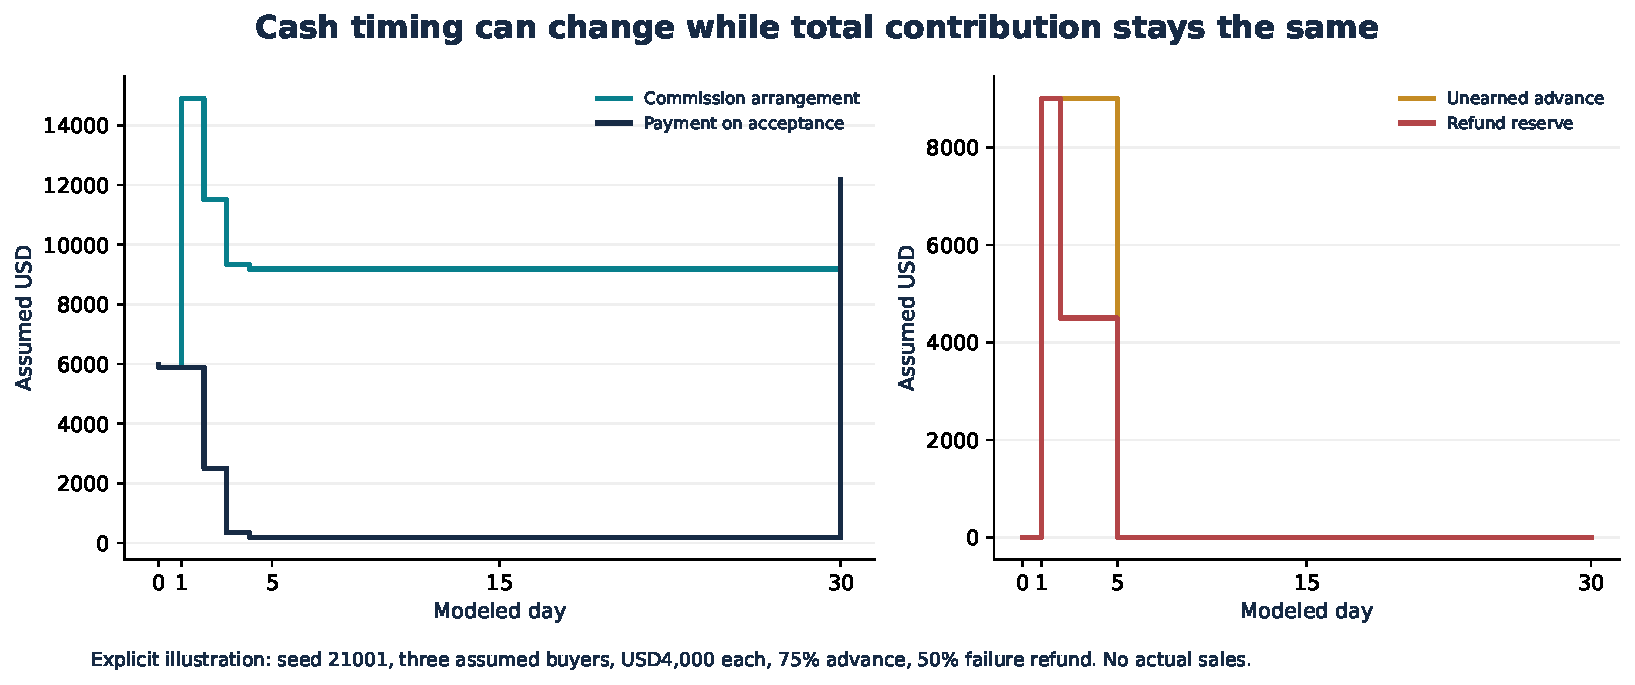
\includegraphics{figures/04_cash_timing.pdf}
\caption{One explicitly selected simulated cash path. Advances, unearned
obligations and reserves are separate from earned contribution.}
\end{figure}

\hypertarget{retention-can-be-rejected-without-denying-useful-capability}{%
\subsection{Retention can be rejected without denying useful
capability}\label{retention-can-be-rejected-without-denying-useful-capability}}

A separate prospective six-horizon admission policy used development
seeds only. Under favorable preexisting-instrument assumptions, its
estimated incremental benefit was USD2,220.94. Proposed new research
construction, initial retention and fresh-recipient transfer totaled
USD2,950. The policy therefore rejected the campaign before
confirmation. The chosen policy's incremental expenditure and
incremental gain are both zero; ordinary production remains available.
The diagnostic charges USD100 of additional upkeep only in horizons that
use the retained arm; it assumes no idle-upkeep charge when expert work
is selected. This favorable maintenance assumption is not an observed
operating cost.

For diagnosis, twenty forced-construction paths then charged the full
initial USD2,800 and USD150 transfer at horizon four, held capacity
constant and capped spendable cash at USD6,000 each horizon. Their mean
final incremental net value was \textbf{−USD1,049.79}, with only two of
twenty paths nonnegative. These hypothetical paths do not
retrospectively admit the rejected campaign or recover profit. The
ordinary library with identical contents and permissions has the same
path; no graph-specific premium is assumed.

This is a concrete stop decision rather than a claim that valuable
skills do not exist. The initial finite benefit upper-bound check was
reachable and the incremental comparison included an efficient expert.
The campaign loses under its stated assumptions. A lower construction
quote, stronger demonstrated transfer or independently evidenced reuse
could justify a new prospectively frozen policy; none is substituted
after seeing these outcomes.

\begin{figure}
\centering
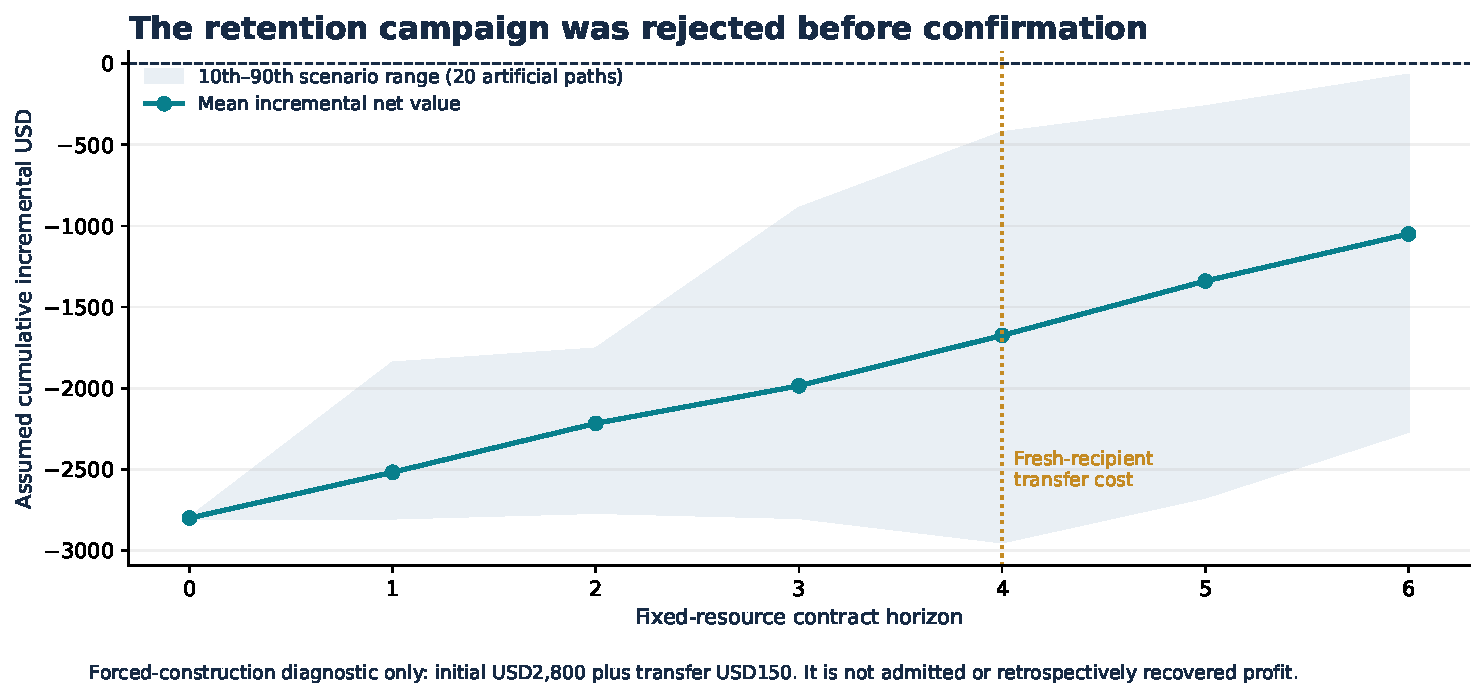
\includegraphics{figures/05_cumulative_net_value.pdf}
\caption{A forced-construction diagnostic after prospective rejection;
it does not recover or admit profit.}
\end{figure}

\begin{figure}
\centering
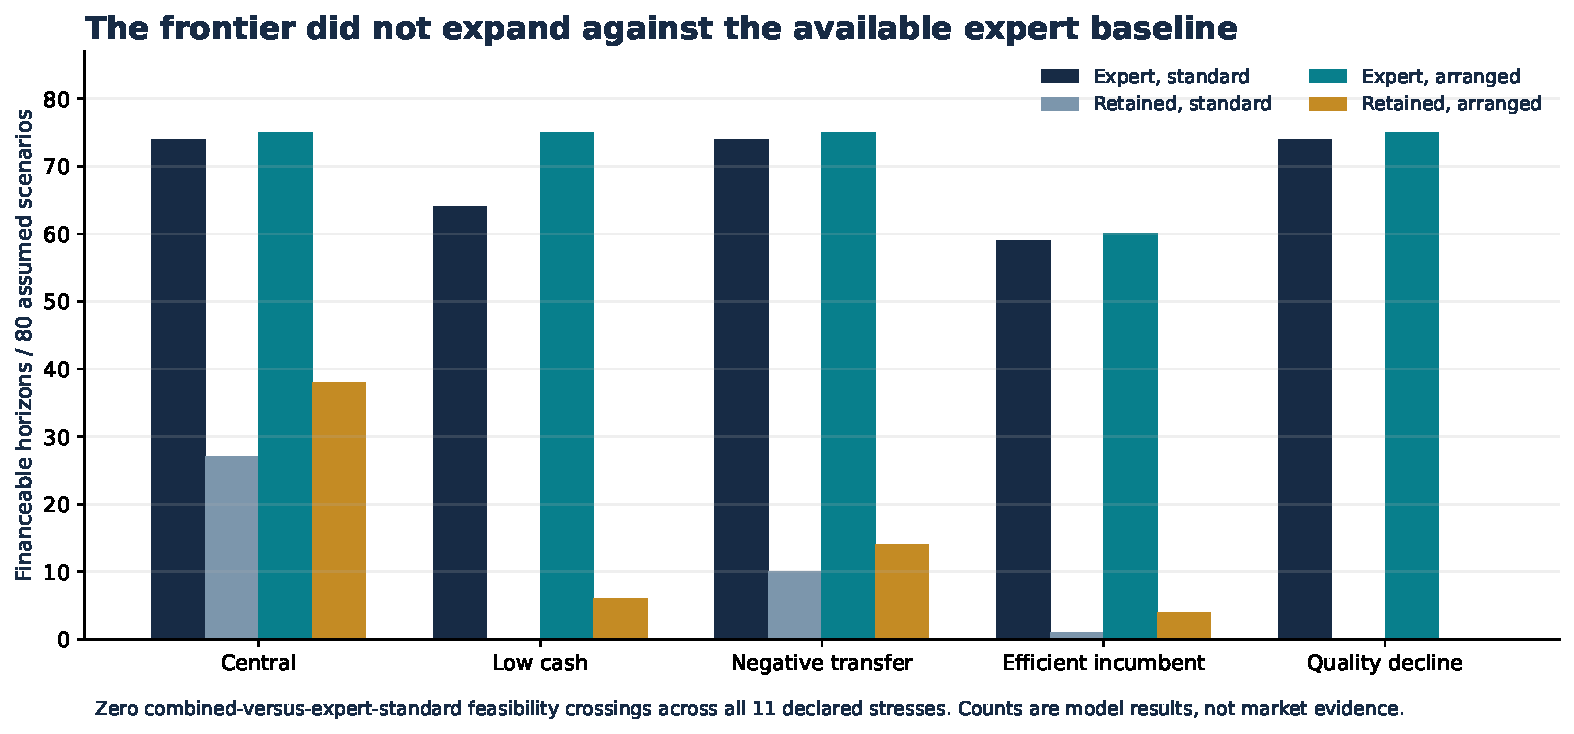
\includegraphics{figures/06_productive_frontier.pdf}
\caption{The modeled productive frontier remains unchanged against the
expert alternative.}
\end{figure}

\hypertarget{what-becomes-possible-next}{%
\section{What becomes possible next}\label{what-becomes-possible-next}}

The executable work changes what a successor can inspect without
reconstructing every reader, reference chain and proof routine. It
exposes a valid permutation-invariant record question, a real
counterexample on a new part and a useful evidence-acquisition mission.
It also leaves a clearer specification for corrected source exports and
later metrology. These are actual computational assets and accepted
scoped outputs, subject to the recorded failures.

The stronger frontier did not move in this edition. Physical report
substitution, individual cross-provider localization and part release
remain unsupported by missing evidence. No new commercial feasibility
crossing was established against the available expert baseline. No
surplus-funded increase in agents, compute or jobs was used to
manufacture compounding. A larger graph, more report fields, a lower
parser runtime or positive hypothetical market size would not change
those conclusions.

This boundary is operationally useful. Produce when the existing expert
service meets acceptance and participation. Construct when a complete
proposal earns its cost and fits cash. Retain or share when expected
recipient reuse justifies the additional qualification and upkeep. Buy
new evidence when an actual unresolved claim requires it. Preserve cash
or stop when those conditions fail. The program does not require every
loop to run.

\hypertarget{operating-blueprint}{%
\section{Operating blueprint}\label{operating-blueprint}}

\hypertarget{a-concrete-initial-offer}{%
\subsection{A concrete initial offer}\label{a-concrete-initial-offer}}

Offer an authorized, bounded inspection-evidence assessment for one
stated part/revision and an agreed set of obligations. Specify the
expected output before intake: a complete source inventory, traceable
conclusions or counterexamples, identified uncertainty, and a
decision-specific acquisition plan. Quote separately for physical
measurements, correction of authoritative exports, new proprietary
adapters, individual feature localization and release support. A
purchase of a complete substitution decision cannot be closed by
renaming an insufficiency report as success.

Obtain the buyer's actual outside option: its configured QIF/PLM chain,
an existing integrator or laboratory, and its ability to defer. The
unfamiliar-packet H estimate is unsuitable for a recipient whose current
system already resolves the question in a few hours. Seek a matched
quote or timed trial before turning any assumed price into a commercial
claim. The research supplies no geographic market-size estimate; USD is
only the model's numeraire. Its six horizons are contract-cycle
scenarios, not a forecast of worldwide demand.

\hypertarget{deliver-expertly}{%
\subsection{Deliver expertly}\label{deliver-expertly}}

Intake can automatically inventory file versions, hashes, schemas, units
and scope, but it cannot invent rights or a missing authority revision.
Execute the smallest useful source and geometry checks. Preserve literal
signs, current standards and parent status. A reviewer checks material
conclusions against source-derived evidence; the need and duration of
residual review are measured when performed, not imposed as arbitrary
routine minutes.

Separate three outputs in every report: numerical entailment, evidence
sufficiency for the requested physical claim, and current permission.
When a claim fails, produce the exact violating value or unresolved
relation, not an unhelpful blanket refusal. When evidence is missing,
ask for the smallest authorized item that could resolve it. Examples are
a corrected units declaration with revision provenance, a relevant
feature mapping, a specimen/lot relation or a task-specific uncertainty
statement. No whole confidential archive is required by default.

Track preparation, tool/model usage, failed attempts, correction,
checking, customer clarification, delivery and support. A low runtime
for the final script is not a complete accepted-service cost. If the
existing configured method is better, use it rather than forcing the
retained tool into every job.

\hypertarget{construct-and-retain-selectively}{%
\subsection{Construct and retain
selectively}\label{construct-and-retain-selectively}}

The potentially shareable asset is generic executable code and its
operating policy, with schemas, dependencies, declared scope, source
provenance, evidence, limitations and upkeep costs. Customer-specific
designs, inspection data, restricted intellectual property, protected
answers and private clarification stay outside the package. Rights to
process a file do not imply rights to redistribute it or train a model
on it.

Admission should inspect whether a hurdle can be satisfied before
purchasing a large evaluation. Bound the plausible benefit from
compatible current or independently evidenced future reuse, subtract
additional assessment, retention, serving and maintenance, and compare
with the recipient's actual baseline. A failed or rejected candidate
still incurs its costs. If a policy is corrected, retain its old
decisions and test the new policy prospectively.

Successful paid delivery may yield candidate expertise. This edition's
actual research is not paid delivery. Its method update is a versioned
operating artifact; it is not weight training or a demonstrated
specialist ASI. A Gym campaign would need an initial policy,
environment, feedback, update rule, budget and resulting version, with
diverse development tasks and independent fresh evaluation. Reward
exploitation, contamination, negative transfer and obsolescence are
explicit rejection conditions. Workflow refinement is an economical
first option; model fine-tuning or reinforcement learning is not assumed
available or necessary.

The frozen economics reject additional retention in the tested finite
portfolio. Accordingly no mandatory Gym or sharing expenditure is
manufactured. Research transfer still tests the mechanism under
separately granted authority, without claiming commercial admission.
Access to a specialist service would preserve service utility; it would
not make each recipient independently possess that specialist's
intelligence.

\hypertarget{participation-and-financing}{%
\subsection{Participation and
financing}\label{participation-and-financing}}

A shared generic adapter can be negotiated across independent private
projects without pooling customer CAD. Each counterparty sees the common
deliverable, its private adaptation, price, rights, timing,
responsibility, refund and support terms. Conditional commitments must
be attractive individually, not merely in aggregate. A shared technical
failure is a correlated event.

An advance creates cash and an obligation together. Finance only against
the spendable portion permitted by the agreed milestone and reserve
rules. Recheck withdrawal and capacity before launch. Keep paid
development, generic qualification and private acceptance distinct.
Collect after the relevant acceptance and expose remaining
receivables/default risk. Never count seed, customer savings, token
issuance or an estimated opportunity value as earned revenue. A positive
expected contribution with unaffordable prefunding is a stop or
renegotiation decision.

\hypertarget{multi-agent-coordination-that-actually-occurred}{%
\subsection{Multi-agent coordination that actually
occurred}\label{multi-agent-coordination-that-actually-occurred}}

The team separated opportunity research, core construction, independent
curation/checking, integration/accounting, and publication. Agents
exchanged an interface contract, source identities and freeze
notifications rather than silently sharing protected answers. The
independent reviewer detected an actionability defect that the core's
own status label did not catch. The integration worker delivered actual
bytes to a separate process and invoked the independent checker. The
hosted method recipients used separate conversations without parent
history and common source/tool ceilings.

This is actual task coordination on a shared host, not institutional
independence or proof that a larger swarm is intrinsically better. No
agent count is treated as commercial gain. The same-content library
matched the graph control. Repository coordination remained in issue
\#4850 with existing owners; no competing registry or production
execution lifecycle was created.

\hypertarget{protected-access-and-intended-token-utility}{%
\subsection{Protected access and intended token
utility}\label{protected-access-and-intended-token-utility}}

For a future admitted, rights-cleared capability, currently eligible
\texttt{*.\allowbreak{}agent.\allowbreak{}agi.\allowbreak{}eth} agents should be able to discover and request
access through the protected network. Eligibility must still be followed
by current recipient, mission, scope, source and authority checks.
Revocation, expiry, Jobs validator roles, governance and settlement
remain authoritative. The present local signature fixtures are not live
ENS authentication, and the native manufacturing scope remains
unqualified.

The intended utility of \$AGIALPHA concerns concrete coordination
mechanisms: funding eligible jobs or budgets, escrow and contractual
settlement, worker and validator incentives, and governed access or
reserves where implemented by the current system. Existing source
implementations and the earlier local-EVM fixtures must not be described
as this edition's live token transactions. {[}3,16{]} Scientific
capability, token access, legal classification, token market value and
enterprise cash profit are different quantities. This study measures no
token valuation and reaches no legal classification conclusion. Its
accounting simulation uses USD and contains no token issuance or
exchange-rate subsidy.

\hypertarget{frontier-model-operation-and-obsolescence}{%
\subsection{Frontier-model operation and
obsolescence}\label{frontier-model-operation-and-obsolescence}}

The hosted team used frontier reasoning with local code execution,
XML/CAD tools, source research and independent correction. The current
official model documents were checked on 27 October 2026.
\texttt{gpt-\allowbreak{}6-\allowbreak{}astra} is the verified reasoning identifier;
\texttt{gpt-\allowbreak{}6.\allowbreak{}1-\allowbreak{}terra} is an available execution/computer-use candidate;
model choice should remain role-dependent and updateable. The verified
standard prices were USD10/1/50 per million input/cached-input/output
tokens for Astra and USD1/0.05/5 for Terra. Longer-context and
service-tier multipliers require their own checks. These are sourced API
prices, not observed billing for this hosted study. {[}11--13{]}

The current hosted interface does not expose a complete served API
snapshot, inference-token ledger or customer billing attribution. No
Terra computer-use experiment or proprietary-weight update was claimed.
ChatGPT Pro is a plan, not an API model identifier or automatic access
entitlement. No weak no-tool substitute is treated as the ceiling of
frontier AI. No measured gain is credited to a model upgrade in the
U/E/E+ comparison. The software pilot and model-default stress both show
why a retained advantage must be requalified as ordinary tools improve.

\hypertarget{before-live-operation}{%
\subsection{Before live operation}\label{before-live-operation}}

The remaining work is concrete: independent prospective engineering
acceptance on genuinely different industrial packets; actual
human/integrator quotes or trials; buyer-specific rights and
source-owner corrections; measured customer interaction, complete
model/tool/support costs and service latency; accepted contracts and
financing commitments; and owner-led production scope and security
qualification. None is satisfied by publishing this research draft. The
next commercial commitment should be a small scoped pilot whose promised
outcome, price, refund rules and acceptance can be reviewed before work
begins.

\hypertarget{interpretation-and-limitations}{%
\section{Interpretation and
limitations}\label{interpretation-and-limitations}}

The work establishes an inspectable construction and a bounded
computational transfer. It does not establish autonomous demand
discovery, a general invention algorithm, independent customer value,
specialist ASI, positive learning Alpha, or commercial compounding. The
original requirements make those distinctions necessary; they are not
reasons to suppress useful narrower results.

The manufacturing data are public, historical and related. Model
contamination cannot be ruled out. The numerical invariance is
established mathematics, and all expert arms may use it. The CAD checker
shares a kernel with the candidate. The source files lack evidence
needed for physical reuse. The initial instrument failed three
useful-report requirements. Native production scope rejects this domain.
The market and cost parameters are uncalibrated hypotheses; the first
observed acceptance result does not validate their assumed quality.
Hosted resource ceilings are matched only in observable calls/output,
and complete costs remain unknown.

These limits identify the next decisive tests. A genuinely unrelated
packet would challenge transfer; a buyer's configured workflow would
challenge added value; a timed accepted-delivery trial would challenge
cost; a signed conditional commitment would challenge participation; and
a cash-prefix ledger with actual payment terms would challenge
financing. A new independent discovery campaign would be needed to test
whether the enterprise has learned to find opportunities more
efficiently. None can be replaced by increasing synthetic sample count.

The \$15 quadrillion projection and intellectual-property superlatives
on the original AGI Alpha vision site are treated as external
promotional claims. They supply no market-size, willingness-to-pay,
asset-value or growth parameter in this study. {[}14{]} We do not
estimate a total addressable market, extrapolate hypothetical savings
across sectors, or count a customer's savings and the enterprise's
revenue as two independent additions to value.

\hypertarget{conclusion}{%
\section{Conclusion}\label{conclusion}}

The opportunity search left behind more than a selected benchmark:
preserved rejections, a current-software falsification, a real
manufacturing evidence instrument, exact semantic counterexamples, an
independently checked recipient handoff and a prospective rule that can
decline further investment.

The most useful transformation is specific. A universal question about
selected records can survive unknown label permutations; a question
about a physical feature or release still needs its missing evidence.
The successor inherits the reader and proof structure while rechecking
meaning and earning current authority. The commercial test is equally
specific: existing expert delivery remains the strong alternative, the
simulated combined offering does not create a new feasibility crossing,
and the tested retention campaign should stop.

That result preserves the AGI Alpha ambition without spending its
conclusion in advance. Profitable delivery can be a foundation; expert
operation can create legitimate advantage; retained instruments can
equip later work. In this edition, what is demonstrated is the
instrument and the discipline needed to distinguish those possibilities
from earned Alpha. The next expansion must be earned through new
evidence.

\hypertarget{authorship-assistance-and-publication-status}{%
\section{Authorship, assistance and publication
status}\label{authorship-assistance-and-publication-status}}

\textbf{Vincent Boucher --- President of MONTREAL.AI.} This exact
attribution is supplied by the commissioning author. Research, code,
analysis, translation and editorial preparation were performed with AI
assistance in this session. The role-separated reviewers are AI agents
on a shared workspace, not independent human peer reviewers. Public
sources, researcher-supplied structures, observed executions,
corrections and simulated quantities are identified separately.

This is a versioned additive research edition, not a software release or
an owner-approved production claim. Browser-readable Markdown, PDF,
editable LaTeX, reproducible code/data, evidence companion, executive
brief and English/French demonstration accompany it. Public draft
publication uses a dedicated source branch and review process. Canonical
Pages/catalogue and release publication remain with their authorized
owners.

\hypertarget{references-and-source-custody}{%
\section{References and source
custody}\label{references-and-source-custody}}

All web-source checks are dated 27 October 2026. Source facts, vendor
capabilities and model documentation are distinguished from this study's
own computations. Complete archive/member hashes and notices appear in
the data manifests.

\begin{enumerate}
\def\labelenumi{\arabic{enumi}.}
\tightlist
\item
  \textbf{Boucher, V. / MONTREAL.AI.} \emph{Transformational
  Intelligence: Learning to Change the Game}. Exact repository edition
  at runtime source freeze, 24 pages.
  \href{https://github.com/MontrealAI/AGI-Alpha-Agent-v0/blob/80b345828f34fd8a6e592977dd17ef37141305f4/docs/Transformational_Intelligence.pdf}{PDF}.
  SHA256 begins \texttt{d7170e8217e3}.
\item
  \textbf{Boucher, V. / MONTREAL.AI.} \emph{Invent the Economy:
  Transformational Intelligence for Creating Viable Markets}. Exact
  repository edition, 22 pages.
  \href{https://github.com/MontrealAI/AGI-Alpha-Agent-v0/blob/80b345828f34fd8a6e592977dd17ef37141305f4/docs/Invent_the_Economy.pdf}{PDF}.
  SHA256 begins \texttt{61e92a47b32c}.
\item
  \textbf{MONTREAL.AI / Writer \#4.} \emph{Transformational Autonomous
  Enterprises: SUCCESSOR Ω Harness}. 23 October 2026 edition, 29
  physical pages.
  \href{https://github.com/MontrealAI/AGI-Alpha-Agent-v0/blob/80b345828f34fd8a6e592977dd17ef37141305f4/docs/papers/transformational-autonomous-enterprises-v1.pdf}{PDF}.
  SHA256 begins \texttt{640cba6e0371}. Historical attribution retained.
\item
  \textbf{NIST.} \emph{Defining the Requirements for Integrating
  Information between Design, Manufacturing, and Inspection}.
  \href{https://www.nist.gov/publications/defining-requirements-integrating-information-between-design-manufacturing-and}{Publication
  record};
  \href{https://pmc.ncbi.nlm.nih.gov/articles/PMC11167730/}{full public
  article}. Existing integration difficulties and experiment context;
  not proof of a current unserved market.
\item
  \textbf{NIST/MTC.} \emph{Design, Manufacturing, and Inspection Data
  for a Three-Component Assembly}.
  \href{https://www.nist.gov/publications/design-manufacturing-and-inspection-data-three-component-assembly}{Publication},
  \href{https://doi.org/10.18434/T4/1503154}{dataset DOI},
  \href{https://nvlpubs.nist.gov/nistpubs/jres/124/jres.124.004.pdf}{J.
  Res. NIST 124, 124.004}. Original archive hash begins
  \texttt{6bc4693f4b07}.
\item
  \textbf{NIST.} \emph{Reference Knowledge Graphs of STEP and QIF Data
  for a Three-Part Box Assembly}.
  \href{https://doi.org/10.18434/M32146}{Dataset DOI},
  \href{https://data.nist.gov/od/ds/mds2-2146/qif-ontology-dataset-V2.zip}{official
  archive}. Archive hash begins \texttt{9ae303335274}. Supplied
  graphs/models are existing baseline assets.
\item
  \textbf{NIST / CCAM.} \emph{Spatial and Temporal Data Alignment from
  Disparate Sources for Feature Association}. NIST GCR 24-050, 2024.
  \href{https://doi.org/10.6028/NIST.GCR.24-050}{DOI},
  \href{https://tsapps.nist.gov/publication/get_pdf.cfm?pub_id=957946}{report}.
  Strong prior art for feature association, not a method invented here.
\item
  \textbf{Capvidia.}
  \href{https://kb.capvidia.com/docs/mbd-ready-for-oem}{MBD Ready for
  OEM}, updated 4 September 2026;
  \href{https://www.capvidia.com/products/comparevidia}{CompareVidia};
  \href{https://www.capvidia.com/solutions}{Solutions}. Advertised
  persistent traceability, model/PMI comparison and integration
  services. No vendor ROI percentage is used as a study parameter.
\item
  \textbf{ZEISS.}
  \href{https://www.zeiss.com/metrology/en/software/zeiss-piweb/data-analysis.html}{PiWeb
  data analysis}. Supplier comparison, sorting, filtering and
  notifications. No scope-matched fixed engineering-service quote
  obtained.
\item
  \textbf{DMSC.} \href{https://qifstandards.org/qif-2-1/}{QIF 2.1 owner
  archive page},
  \href{https://qifstandards.org/wp-content/uploads/2015/03/QIF-2.1.zip}{exact
  archive}. \texttt{QIFLibrary/\allowbreak{}Units.\allowbreak{}xsd} SHA256
  \texttt{2d46993e\allowbreak{}49300841\allowbreak{}e66fc05c\allowbreak{}35dafbcb\allowbreak{}63ac8085\allowbreak{}e9c9c8cb\allowbreak{}c8670e97\allowbreak{}c13a5fbd}.
  DMSC copyright/permission notice accompanies redistributed schema
  bytes; this material is not relicensed as Apache or public domain.
\item
  \textbf{OpenAI.}
  \href{https://developers.openai.com/api/docs/models/gpt-6-astra}{GPT-6
  Astra model documentation}. Current API
  identifier/capabilities/prices, distinct from hosted study telemetry.
\item
  \textbf{OpenAI.}
  \href{https://developers.openai.com/api/docs/models/gpt-6.1-terra}{GPT-6.1
  Terra model documentation}. Role-appropriate execution/computer-use
  candidate; not an executed Terra trial here.
\item
  \textbf{OpenAI.}
  \href{https://developers.openai.com/api/docs/pricing}{API pricing}.
  Standard token rates and service/context qualifications require
  current verification before operation.
\item
  \textbf{AGI Alpha Agent vision.}
  \href{https://agialphaagent.com/}{agialphaagent.com}. Motivation only.
  The quoted USD15 quadrillion and IP superlatives are external
  promotional claims, not validated findings or forecast inputs.
\item
  \textbf{Scientific software incident and version controls.}
  \href{https://github.com/pydata/xarray/issues/10840}{Xarray issue
  10840},
  \href{https://github.com/zarr-developers/zarr-python/issues/3516}{Zarr
  issue 3516},
  \href{https://zarr.readthedocs.io/en/stable/api/zarr/storage/index.html}{official
  stable storage documentation}. Exact packages, attempts and artifacts
  are frozen in the runtime pilot dossier. The executed current-version
  pass is our observation, not inferred from a release note.
\item
  \textbf{MONTREAL.AI AGI-Alpha-Agent-v0.}
  \href{https://github.com/MontrealAI/AGI-Alpha-Agent-v0}{Repository},
  \href{https://github.com/MontrealAI/AGI-Alpha-Agent-v0/issues/4850}{coordination
  issue 4850},
  \href{https://github.com/MontrealAI/AGI-Alpha-Agent-v0/issues/4850\#issuecomment-6447631102}{this
  lane's selection update}. Research parent and immutable runtime bridge
  identities appear in the reproducibility manifest.
\item
  \textbf{NIST.}
  \href{https://www.nist.gov/services-resources/software/step-file-analyzer-and-viewer}{STEP
  File Analyzer and Viewer},
  \href{https://github.com/usnistgov/SFA}{current source repository}.
  Existing geometry/PMI inspection belongs in the expert baseline.
\item
  \textbf{NIST.} \href{https://www.nist.gov/open/license}{Copyright,
  Fair Use, and Licensing Statements}, updated 24 June 2025. Apply
  dataset-specific notices and distinguish third-party/extramural
  material; do not assign a blanket license to every archive member.
\end{enumerate}

The full opportunity dossier retains additional primary sources for
deferred and rejected candidates, with query records, archive
identities, source limitations and the original decision chronology.
Those sources motivate selection; they are not evidence that a novel
market has been created.

\end{document}
